\documentclass{beamer}

\mode<presentation>

{
 \usetheme{AnnArbor}   
 \usecolortheme{crane}
 \usefonttheme{serif} 
 \setbeamertemplate{navigation symbols}{}
 \setbeamertemplate{caption}[numbered]
 \setbeamertemplate{background canvas}[vertical shading][bottom=red!50,top=yellow!30]

  %\setbeamertemplate{background canvas}{\includegraphics         [width=\paperwidth,height=\paperheight]{nombre_del_fondo.jpg}}
}

\usepackage[spanish]{babel}
\usepackage[utf8]{inputenc}
\usepackage{amsmath, amsfonts}
\usepackage{graphicx}


\title[Universidad de la Laguna]{Integración Simpson}

\author[]{Cristina González Marrero\\
          Ashneet Khandpur Singh\\
          Lorena Morales Pérez}

\institute{Grupo 2-G}

\date{17 de Mayo de 2013}


\begin{document}
 
 \begin{frame}
   \titlepage
 \end{frame}


\begin{frame}{Índice}
  \tableofcontents[pausesections]
\end{frame}

\section{Introducción}
\begin{frame}{Introducción}
  \hskip 4cm{\colorbox{yellow}{$f(x)=\frac{x^3}{1+x^{1/2}}, x \in [1, 2]$}}
  \vskip 1cm
  \begin{block}{Definición}
    \textcolor{red}{La regla de Simpson nos proporciona una estimación más exacta  de una integral aplicando polinomios de orden superior para conectar los puntos.}
  \end{block}
\end{frame}

\section{Motivación y objetivos}
\begin{frame}{Motivación y objetivos}
  \begin{itemize}
    \item Objetivo principal\\
    \vskip 0.5cm
    \parindent 0.5cm Comprender el funcionamiento del método de simpson aplicado a funciones, asi como acotar el error cometido en la integración numérica a través de éste
  \end{itemize}
\end{frame}
 

\section{Fundamentos teóricos}
\begin{frame}{Fundamentos teóricos}
La regla o método de Simpson (nombrada así en honor de Thomas Simpson) es un método de integración numérica que se utiliza para obtener la aproximación de la integral:
\[\int_a^{b}f(x) \: dx \approx \frac{b-a}{6} \Bigg[f(a)+4f\Big(\frac{a+b}{2}\Big)+f(b)\Bigg]\]
\end{frame}

\begin{frame}{Error}
La ecuación anterior tiene un error asociado de:
 \[E_t = \frac{-1}{90}h^5 f^4(\xi)\]
El error asociado a la regla de Simpson nos indica que este método es más exacto que otros métodos de integración como la regla del trapecio.\end{frame}

\section{Procedimientos experimentales}
\begin{frame}{Procedimientos experimentales}
 \begin{itemize}
   \item Descripción de los experimentos:
    
    \parindent=0.5cm Utilizando la fórmula simple y compuesta se ha calculado el error de la aproximación y el tiempo que tarda nuestro ordenador en calcular dicho cálculo.
   \item Descripción del material\\
    CPU speed: 2267.448 Hz
 \end{itemize}
\end{frame}

\section{Resultados obtenidos}
\begin{frame}{Resultados}
  \begin{itemize}
    \item Resultados obtenidos \\
      \begin{table}
	\centering
	\begin{tabular}{||c|c c c||}
	  \hline
	  \hline
	  N & Integral & Error & Tiempo  \\
	  \hline
	  10     & 1.2672   & -0.3798 & 0.00117  \\
	  100    & 1.3044   & -0.3426 & 0.00503  \\
	  1000   & 1.3082   & -0.3388 & 0.1333   \\
	  10000  & 1.3086   & -0.3384 & 1.1772   \\
	  100000 & 1.3086   & -0.3384 & 11.8899  \\
	  \hline
	  \hline
	\end{tabular}
	\caption{\label{tab:widgets}Error y tiempo.}
     \end{table}
  \end{itemize}
\end{frame}


\begin{frame}{Gráfica función}
  \begin{figure}[ptb]
    \begin{center}
      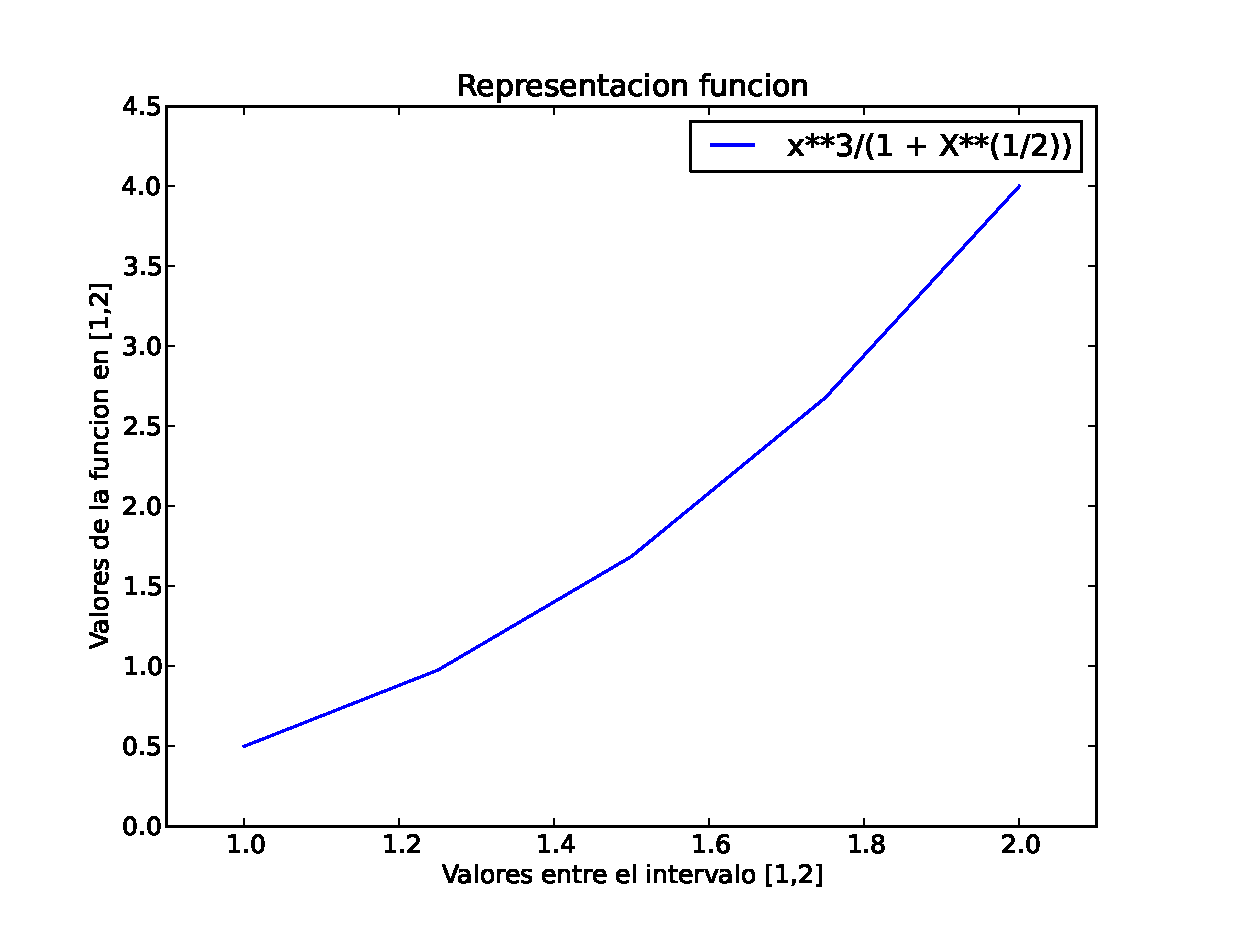
\includegraphics[width=0.75\textwidth]{tmp2.eps}
      \caption{Gráfica de la función}
      \label{fig:1}
    \end{center}
  \end{figure}
\end{frame}  
  
\begin{frame}
  \begin{figure}[h]
    \begin{center}
      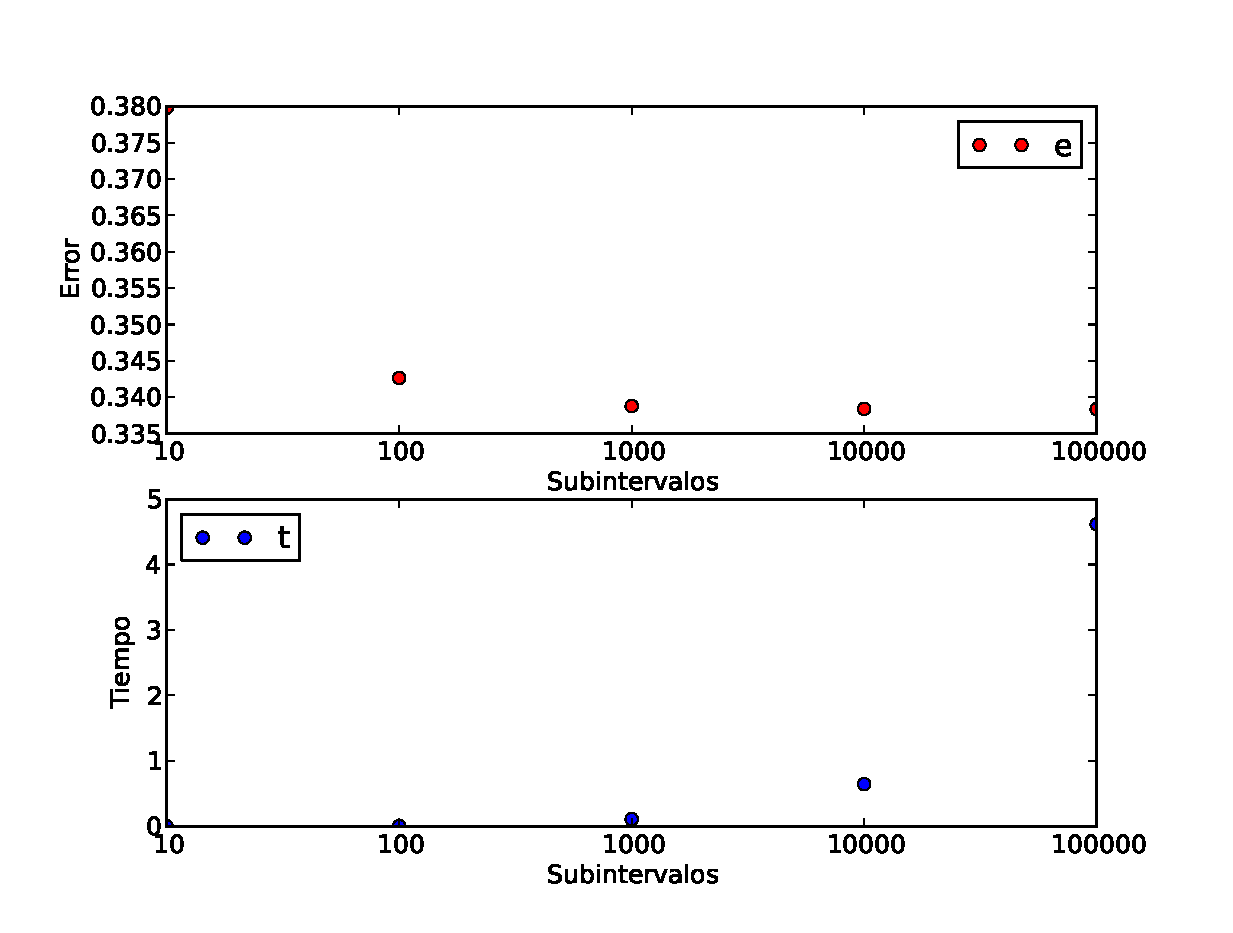
\includegraphics[width=0.75\textwidth]{errortiemp.eps}
      \caption{Gráfica del error y tiempo}
      \label{fig:2}
    \end{center}
  \end{figure}
\end{frame}

\section{Conclusiones}
\begin{frame}{Conclusión}
  \frametitle{Conclusiones}
  En conclusión, la regla de Simpson para el cálculo de integrales es muy apropiada, pero sobretodo el empleo de la fórmula 
compuesta, ya que nos permite elegir el número subintervalos y calcular la integral en cada uno de ellos, de manera que se 
obtiene un valos bastante aproximado de la integral. Aunque, debemos tener en cuenta que cuánto mayor es el número de intervalos,
más tarda el programa en realizar el cálculo. 
  
\end{frame}


\begin{frame}
  \frametitle{Bibliografía}
  \scriptsize
  \begin{thebibliography}{9}
  \bibitem{label}
   www.wikipedia.org
  \bibitem{label1}
  www.slideshare.net
  \bibitem{label2}
  www.metodos.fam.cie.uva.es
  \bibitem{label3}
  Python para todos. Raúl González Duque. Mundo geek. GPL. zootropo en gmail. 
  \bibitem{label4}
  www.aristarco.com.es
  \bibitem{label5}
  es.scribd.com
  \bibitem{label6}
  www.artofproblemsolving.com
  \end{thebibliography}
\end{frame}

\end{document}